Incorporating candidate words with an attention mechanism into the character-based BiLSTM-CRF architecture, as shown in Figure~\ref{fig:base-model}, could yield superb segmentation performance \cite{higashiyama-etal-2019-incorporating}.
%
An attention mechanism has the advantage of being flexible for use with additional linguistic knowledge such as CCs and subword units.
%
Thus, we use the concept of CC with an attention mechanism in character-based word segmentation, as shown in Figure \ref{fig:main-model}, by extending the BiLSTM-CRF architecture with word attention from \citeA{higashiyama-etal-2019-incorporating}.

\begin{figure}[ht]
    \centering
    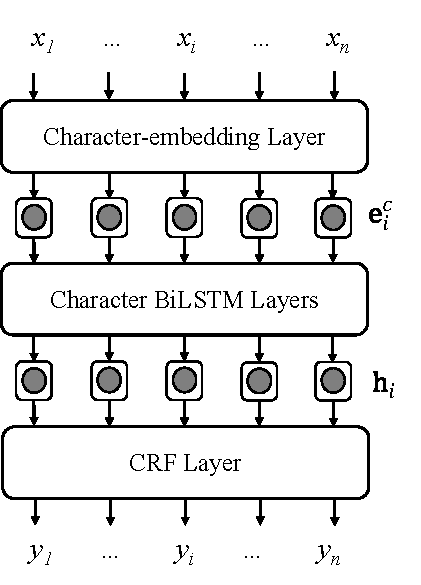
\includegraphics[width=0.3\textwidth]{figures/fig-base-model.pdf}
    \caption{Character-based BiLSTM-CRF architecture as our Baseline where $x$ and $y$ represent each character from an input sequence and a predicted label for each character, respectively. $\textbf{e}^{c}$. indicates an embedding representation for each character, and $\textbf{h}$ presents BiLSTM-encoded representation for each character.}
    \label{fig:base-model}
\end{figure}
%
Our model estimates \textit{CC-integrated character vectors} ${\textbf{z}}$ are incorporated on top of \textit{word-integrated character vectors} ${\textbf{g}}$, which are almost identical in architecture.
%
We discuss the major components of our model, i.e., the character-embedding layer, word- and CC-embedding layers, BiLSTM layers for character representation, attention integrations with the BiLSTM layers for integrated representations, CRF layer, and optional BERT layers.
%
\begin{figure}[ht]
    \centering
    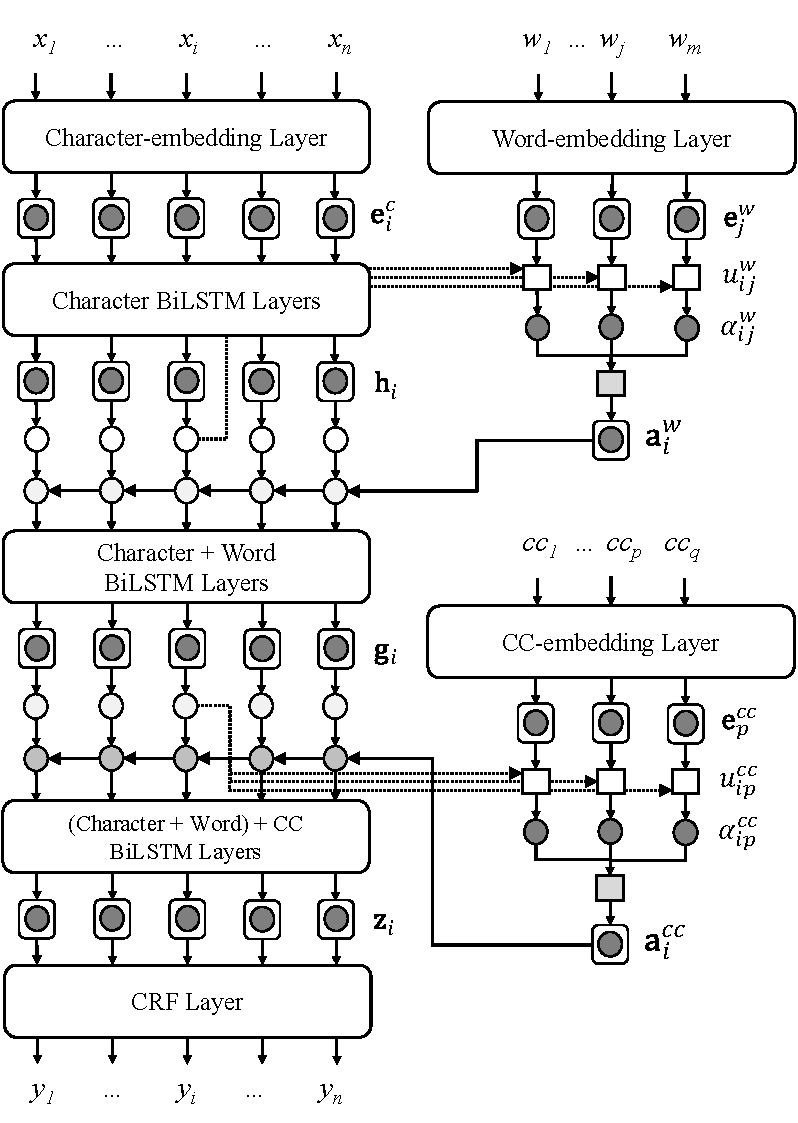
\includegraphics[width=0.58\textwidth]{figures/fig-main-model.pdf}
    \caption{Our model integrating word and CC attentions into character-based BiLSTM-CRF architecture.}
    \label{fig:main-model}
\end{figure}
%

\subsection{Character-embedding Layer}
Given a sentence $s$ with $n$ characters that can be represented as $x_{1:n} \equiv (x_1, x_2, \dots, x_n)$, each character $x_{i} \in x_{1:n}$ is transformed into a character embedding $\textbf{e}_{i}^{c}$ of a $d_{c}$-dimensional vector using lookup-table operation \cite{Bengio2003,Collobert2011}.
%
The lookup table is defined as $\text{E}^{c} \in \mathbb{R}^{d_{c} \times |V_c|}$, where $d_{c}$ denotes the dimension of embeddings and $V_c$ denotes a character vocabulary.
%
% Each character embedding $\textbf{e}_{i}^{c}$ can be obtained from the corresponding column in the lookup table $\text{E}_{1:n}^{c}$.

\subsection{Word- and CC-embedding Layers}\label{section:word-cc-embed}
Using the word embedding layer as an example, let $V_{w}$ be a word vocabulary.
%
Given the character sequence $x_{1:n}$, words are searched on the basis of $V_{w}$ within a maximum word length $K$ of the character subsequence. 
% 
A candidate word list $\mathcal{W}_{x}$ $\equiv (w_{1}, \dots, w_{m})$ of size $K$ with $m$ candidate words is then obtained, as shown in Figure~\ref{fig:main-model}.
%
Each word $w_{j} \in \mathcal{W}_{x} \subseteq V_{w}$ is transformed into a word embedding $\textbf{e}^{w}$ of a $d_{w}$-dimensional vector. 
%
The word-embedding matrix is defined as $\text{E}^{w} \in \mathbb{R}^{d_{w} \times |V_{w}|}$, where $d_{w}$ denotes the dimension of embeddings.
%
This procedure is also applied to obtain a candidate CC list $\mathcal{CC}_{x}$, which is transformed into a CC-embedding layer $\textbf{e}^{cc}$ of a $d_{cc}$-dimensional vector. 
%
The CC-embedding matrix is defined as $\text{E}^{cc} \in \mathbb{R}^{d_{cc} \times |V_{cc}|}$, where $d_{cc}$ denotes the dimension of embeddings and $V_{cc}$ denotes a CC vocabulary.

\subsection{BiLSTM Layers for Character Representation}\label{section:bilstm-for-char}
The character embedding sequence $\textbf{e}_{1:n}^{c}$ is provided to the BiLSTM \cite{Hochreiter1997,Gers2000} layers to contextually acquire \textit{character context vectors} $\textbf{h}_{1:n}$.
%

A current character context vector $\textbf{h}_{i}^{l} \in \textbf{h}_{1:n}^{l}$ of the $l$-th layer BiLSTM can be computed bidirectionally:
%
\begin{equation}
    \begin{split}
        \textbf{h}^{l}_{i} &= \text{BiLSTM}(\textbf{h}^{l-1}_{1:n}, i) \\
        & \equiv \text{LSTM}_f(\textbf{h}^{l-1}_{1:n}, i) \\
        & \oplus \text{LSTM}_b(\textbf{h}^{l-1}_{n:1}, n-i+1),
    \end{split}
    \label{eq:bilstm}
\end{equation}
where $\textbf{h}^{0}_{1:n} = \textbf{e}_{1:n}^{c}$, $\text{LSTM}_{f}$ denotes forward LSTM, $\text{LSTM}_{b}$ denotes backward LSTM, $\oplus$ denotes concatenation, and $\textbf{h} \in \mathbb{R}^{2d_{r}}$ and $d_{r}$ are hyperparameters.


\subsection{Attention Integrations with BiLSTM Layers for Integrated Representations}\label{section:attn-integration}
We use two attention integrations, including word attention and CC attention, to respectively estimate a \textit{word-integrated summary vector} $\textbf{a}_{i}^{w}$ and \textit{CC-integrated summary vector} $\textbf{a}_{i}^{cc}$ for each character in the character sequence.
%
These integrations, which are equal in architecture, accordingly summarize the relationship among characters, words, and CCs.
%

We apply the composition function \textit{weight concatenation} (WCON) \cite{higashiyama-etal-2019-incorporating,higashiyama-2022-wordseg} to estimate both summary vectors. 
%.
This function produces a word-integrated summary vector on the basis of the relationship between a character and their corresponding candidate words.
%
It also can be used to implicitly produce a CC-integrated summary vector on the basis of the relationship between the character with its corresponding candidates words and candidate CCs.

Starting with word-attention integration, we estimate the word-importance score $u_{ij}^{w}$ and word-attention weight $\alpha_{ij}^{w}$ on the basis of the character context vector $\textbf{h}_{i}$ and candidate word embedding $\textbf{e}_{j}^{w}$ as
% %
\begin{equation}
    u_{ij}^{w} = \textbf{h}_i^{T}W_{a}^{w}\textbf{e}_{j}^{w},
    \label{eq:word-important}
\end{equation}
%
\begin{equation}
    \alpha_{ij}^{w} = \frac{\delta_{ij}\exp(u_{ij}^{w})}{\sum_{k=1}^{m}\delta_{ik}\exp(u_{ik}^{w})},
    \label{eq:word-attn-weight}
\end{equation}
%
where $W_{a}^{w} \in \mathbb{R}^{2d_{r} \times d_{w}}$ denotes a trainable weight matrix and $\delta_{ij} \in \{0,1\}$ indicates whether character $x_{i}$ is included in candidate word $w_{j}$.
%
The word-integrated summary vector $\textbf{a}_{i}^{w}$ for character $x_{i}$ can be calculated as
%
\begin{equation}
    \textbf{a}_{i}^{w} = \text{WCON}^{w}(x_{i}, \{w_{j}\}_{j=1}^{m}) {=} \bigoplus_{l=1}^{L^{w}}\alpha_{i,i_{l}}^{w}\textbf{e}_{i_{l}}^{w},
    \label{eq:wcon}
\end{equation}
%
where \{$w_{j}$\} = $\mathcal{W}_{x}$. 
%
Let $K^{w}$ be the maximum word length, $L^{w} = \sum_{k=1}^{K^{w }}k$, $\bigoplus$ denote concatenation, and $i_{l}$ is the corresponding index of candidate word list $\mathcal{W}_{x}$ for character $x_{i}$ that is $\{w^{\prime}_{1},\dots,w^{\prime}_{L^{w}}\} \equiv \bigcup_{k=1}^{K^{w}}\bigcup_{s=-k+1}^{0}\{x_{i+s:i+s+k-1}\}$.
%
Note that a zero vector is applied to Equation \ref{eq:wcon} when $w^{\prime}_{l} \notin V_{w}$.
%

For instance, to compose the list of words $w^{\prime}_{4}$ containing a character $x_{4}$ for estimating the word-importance score $u^{w}_{4,j}$, the word-attention weight $\alpha^{w}_{4,j}$, and the summary vector $\textbf{a}^{w}_{4}$, let the candidate words list $\mathcal{W}_{x} = \{w_{1},\dots,w_{8}\}$, maximum word length $K^{w} = 4$, and $L^{w} = \sum_{k=1}^{K^{w }}k = 10$, the procedure can be performed as follows:
%
\begin{equation}
    \begin{split}
        w^{\prime}_{4} &= \bigcup_{k=1}^{4}\bigcup_{s=-k+1}^{0} \{x_{4+s:4+s+k-1}\} \\
        & = \{x_{4:4},x_{4:3},x_{4:5},x_{2:4},x_{3:5},x_{4:6},x_{1:4},x_{2:5},x_{3:6},x_{4:7}\}.
    \end{split}
    \label{eq:wcon-x4}
\end{equation}
where the words $x \in w^{\prime}_{4}$ containing in train vocabulary will be used.
%

We then use the BiLSTM layers for transforming the word-integrated summary vectors $\textbf{a}^{w}$ into word-integrated character vectors $\textbf{g}$. 
%
The operation of word-integrated character vector $\textbf{g}_{i}$ is computed using the BiLSTM layers on the basis of word-integrated summary vector $\textbf{a}_{i}^{w}$ with its corresponding character context vector $\textbf{h}_{i}$ as 
%
\begin{equation}
    \textbf{g}_{i} = \text{BiLSTM}(\textbf{h}_{i}\oplus\textbf{a}_{i}^{w}).
    \label{eq:wcon-concat}
\end{equation}
%

However, the candidate CCs that correspond to the character are used on top of $\textbf{g}_{i}$ as
%

\begin{gather}
    u_{ip}^{cc} = \textbf{g}_i^{T}W_{a}^{cc}\textbf{e}_{p}^{cc}, \label{eq:ccwcon-score}\\
    \alpha_{ip}^{cc} = \frac{\delta_{ip}\exp(u_{ip}^{cc})}{\sum_{k=1}^{q}\delta_{ik}\exp(u_{ik}^{cc})},
\end{gather}
%
where $W_{a}^{cc} \in \mathbb{R}^{4d_{r} \times d_{cc}}$ denotes a trainable weight matrix and $\delta_{ip} \in \{0,1\}$ indicates whether character $x_{i}$ is included in the candidate CC $cc_{p}$.
%
The CC-integrated summary vector $\textbf{a}_{i}^{cc}$ for character $x_{i}$ can be calculated as
\begin{equation}
    \textbf{a}_{i}^{cc} = \text{WCON}^{cc}(x_{i}, \{cc_{p}\}_{p=1}^{q}) {=} \bigoplus_{l=1}^{L^{cc}}\alpha_{i,i_{l}}^{cc}\textbf{e}_{i_{l}}^{cc},
    \label{eq:ccwcon}
\end{equation}
%
where \{$cc_{p}$\} = $\mathcal{CC}_{x}$. 
%
Let $K^{cc}$ is the maximum CC length, $L^{cc} = \sum_{k=1}^{K^{cc}}k$, and $i_{l}$ is the corresponding index of potential CC list $\mathcal{CC}_{x}$ for character $x_{i}$, which is represented by $\{cc^{\prime}_{1},\dots,cc^{\prime}_{L^{cc}}\} \equiv \bigcup_{k=1}^{K^{cc}}\bigcup_{s=-k+1}^{0}\{x_{i+s:i+s+k-1}\}$.
%
A zero vector is applied to Equation \ref{eq:ccwcon} when $cc^{\prime}_{l} \notin \mathcal{V}_{cc}$.

Next, we use additional BiLSTM layers to transform the CC-integrated summary vectors $\textbf{a}^{cc}$ into CC-integrated character vectors $\textbf{z}$ on the basis of a cluster-integrated summary vector $\textbf{a}_{i}^{cc}$ and its corresponding word-integrated character vector $\textbf{g}_{i}$ as 
%
\begin{equation}
    \textbf{z}_{i} = \text{BiLSTM}(\textbf{g}_{i}\oplus\textbf{a}_{i}^{cc}).
    \label{eq:ccwcon-concat}
\end{equation}
%
A CRF is finally used to estimate the probability of the optimal label sequences $y$.

\subsection{CRF Layer}
A CRF \cite{Lafferty2001} along with explicitly considering the correlations between adjacent labels has been successfully applied for sequence-labeling-related tasks \cite{Collobert2011}.
%
Let $A \in \mathbb{R}^{|T| \times |T|}$ be a transition matrix for correlations between adjacent labels, where $T$ denotes a set of all possible label sequences, for instance, $T = \{B, I, E, S\}$.
%
The CC-integrated character vector $\textbf{z}_{i}$ is transformed into an un-normalized label score $\textbf{s}_{i}$ of the $|T|$-dimensional vector for character $x_i$ as
%
\begin{equation}
    \textbf{s}_i = W_{s}\textbf{z}_{i} + \textbf{b}_{s},
\end{equation}
where $W_{s} \in \mathbb{R}^{|T| \times 4d_{r}}$ denotes a trainable weight matrix, and $\textbf{b}_{s} \in \mathbb{R}^{|T|}$ denotes a trainable bias. 
%
Given the input sequence $x_{1:n}$, the corresponding scores for the label sequence $y_{1:n}$ are computed on the basis of transition matrix $A$ and the segmentation label scores $\textbf{s}$ as follows:
\begin{equation}
    \text{score}(x, y) = \sum_{i=1}^{n}(A_{y_{i-1},{y_i}} + \textbf{s}_i[y_{i}]).
\end{equation}
%
The probability of the label sequence can then be obtained as
%
\begin{equation}
    P(y|x) = \frac{\text{score}(x,y)}{\sum_{y' \in T^{n}}\text{score}(x,y')}.
\end{equation}
%
We can obtain the optimal label sequence $y^{\star}$ by maximizing the sentence score with the Viterbi algorithm:
%
\begin{equation}
    y^{\star} = \text{argmax}_{y \in T^{n}}\text{score}(x,y).
\end{equation}
%
The loss function $\mathcal{L}$ is minimized by back propagation during the training process:
%
\begin{equation}
    \mathcal{L}(x,y) = - \log P(y|x).
\end{equation}

\subsection{BERT Layers}
In this work, we use BERT layers for comparing with BiLSTM-based models. 
%
$\text{BERT}_{base}$ layer\footnote{https://huggingface.co/bert-base-multilingual-cased} is used to extract three types of representation, including contextual-character-, word-, and CC-representation.
%
Concretely, we replace the BiLSTM layers for character representation in Section \ref{section:bilstm-for-char} with BERT-encoder layer to compute the \textit{character context vectors} $\textbf{h}_{1:n}$ that can be represented in \ref{fig:bert-model}. 
%
The current character context vector $\textbf{h}_{i}$ can be computed: 
\begin{equation}
    \textbf{h}_{i}^{0} = {\textbf{e}^{c}}_{i} + {\textbf{e}^{p}_{i}},
\end{equation}

\begin{equation}
    \textbf{h}_{i}^{l} = \text{Transformer}(\textbf{h}_{i}^{l-1}),
\end{equation}
%
where $l = \{1, 2, \dots, L\}$, which is the number of transformer layers \cite{Vaswani2017}. $\textbf{e}^{c}$ is the embedding obtained from the BERT-embedding layer while $\textbf{e}^{p}$ is the positional embedding.
%
Because we adopt $\text{BERT}_{base}$, $L=12$. $e^{c} \in \mathbb{R}^{d_{c} \times |V_{\text{BERT}}|}$, where $d_{c} = 768$, and $V_{\text{BERT}}$ denotes the vocabulary in $\text{BERT}_{base}$.
%
For the word- and CC-representation, which can be referred in \ref{section:word-cc-embed}, we straightforwardly obtain their representations from the embedding layer of BERT. 
%
In other words, word- and cc-embedding layer (as well as subword-embedding layer) are replaced with BERT-embedding layer.
%
By using the BERT embedding layers, the word- and CC-embedding matrices are defined as $\text{E}^{w} \in \mathbb{R}^{d_{w} \times |V_{\text{BERT}}|}$ and $\text{E}^{cc} \in \mathbb{R}^{d_{cc} \times |V_{\text{BERT}}|}$, where $d_{w}=768$, $d_{cc}=768$.
%
Finally, the BERT-pooler layer and CRF layer are used to conditionally project the BERT representations from its encoder layers into the optimal label sequences $y^{\star}$.

\begin{figure}[ht]
    \centering
    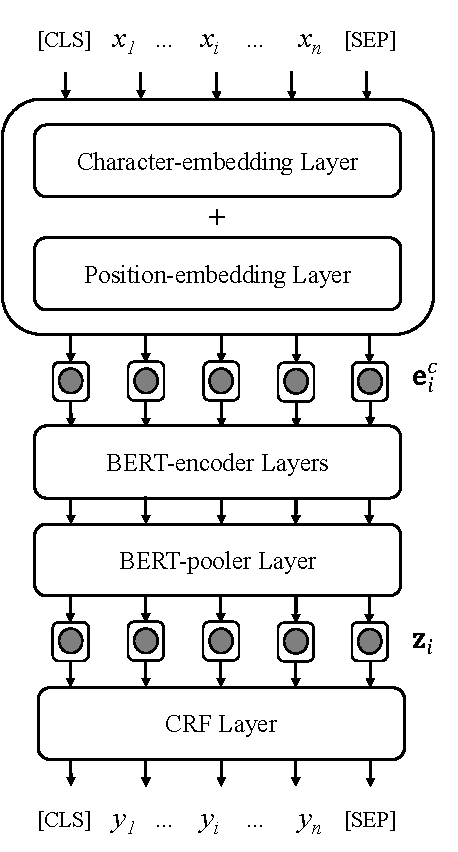
\includegraphics[width=0.35\textwidth]{figures/fig-bert-ext-model.pdf}
    \caption{Character-based word-segmentation model incorporated with BERT pre-trained model.}
    \label{fig:bert-model}
\end{figure}